% docx2tex --- ``Garbage In, Garbage Out''
%
% docx2tex is Open Source and
% you can download it on GitHub:
% https://github.com/transpect/docx2tex
%
\documentclass{article}
\usepackage{graphicx}
\usepackage{hyperref}
\usepackage{multirow}
\usepackage{tabularx}
\usepackage{color}
\usepackage{amsmath}
\usepackage{amssymb}
\usepackage{amsfonts}
\usepackage{amsxtra}
\usepackage{wasysym}
\usepackage{isomath}
\usepackage{mathtools}
\usepackage{txfonts}
\usepackage{upgreek}
\usepackage{enumerate}
\usepackage{tensor}
\usepackage{pifont}
\usepackage{float}
\usepackage{fancyhdr}
\usepackage{lastpage}
\usepackage{incgraph}
\usepackage{changes}
\usepackage{pdfpages}


\usepackage[letterpaper, margin=1in, headheight=47pt]{geometry}

% No paragraph indent
\setlength{\parindent}{0cm}
% Bigger paragraph skips
\setlength{\parskip}{0.25cm}

% TEX Gyre Adventor font (looks pretty nice)
\renewcommand*\rmdefault{qag}

\pagestyle{fancy}

\lhead{}
\chead{}
\rhead{
\includegraphics[width=8cm]{media/image15.png}}
\renewcommand{\headrulewidth}{0pt}
%\renewcommand{\topmargin}{-20pt}

\rfoot{Page \textbf{\thepage} of \textbf{\pageref{LastPage}}}
\lfoot{\textit{Final Rules as of \today}}
\cfoot{}

% First page
\fancypagestyle{firststyle}{%
  \fancyhf{}
  \fancyfoot[L]{\textit{Draft as of \today}}
  \fancyfoot[R]{Page \textbf{\thepage} of \textbf{\pageref{LastPage}}}
}

\definechangesauthor[color=red]{TC}
\setdeletedmarkup{\footnote{In previous version of the rules this was ''\emph{#1}''}}
\setauthormarkup{}

\title{\vspace{-5ex}RoboCupJunior Soccer Rules 2018\vspace{-5ex}}
\date{\vspace{-2ex}}
%\date{Draft as of \today}

\definecolor{color-1}{rgb}{1,1,1}
\definecolor{color-2}{rgb}{0,0,0.5}
\definecolor{color-3}{rgb}{0.07,0.33,0.8}
\definecolor{color-4}{rgb}{0.13,0.13,0.13}
\definecolor{red}{rgb}{1,0,0}
\definecolor{color-6}{rgb}{0,0,1}



\begin{document}
\maketitle
\thispagestyle{firststyle}

\textbf{Soccer Technical Committee 2018:}

\resizebox{0.45\textwidth}{!}{
\begin{tabular}{lr}
    Sarit Salzman             & Israel\\
    James Riley               & Australia\\
    Javier E. Delgado Moreno  & Mexico \\
    Michael Sloan Warren      & USA\\
    Felipe Nascimento Martins & Netherlands\\
    Marek \v{S}uppa           & Slovakia (CHAIR)\\
\end{tabular}}

These are the official Soccer rules for RoboCupJunior 2018. They are released
by the RoboCupJunior Soccer Technical Committee. The English version of these
rules has priority over any translations. \textcolor{red}{\textbf{Items in red
represent significant rules changes introduced this year.}}

Teams are advised to check the RoboCupJunior Soccer site
\href{http://rcj.robocup.org/soccer.html}{http://rcj.robocup.org/soccer.html}
for OC (Organizational Committee) procedures and requirements for the
international competition. Each team is responsible for verifying the latest version of the
rules prior to competition.

\section*{Preface}

In the RoboCupJunior soccer challenge, teams of young engineers design, build,
and program two fully autonomous mobile robots to compete against another team
in matches. The robots must detect a ball and score into a color-coded goal on
a special field that resembles a human soccer field.

To be successful, participants must demonstrate skill in programming, robotics,
electronics and mechatronics.  Teams are also expected to contribute to the
advancement of the community as a whole by sharing their discoveries with other
participants and by engaging in good sportsmanship,regardless of culture, age or
result in the competition. \textbf{All are expected to compete,
learn, have fun, and grow.}

RoboCupJunior Soccer consist of two sub-leagues:

\textbf{``Soccer Open''} and \textbf{``Soccer Lightweight''}. These rules apply
for both sub-leagues. There are two main differences between the two leagues.

\textbf{``Soccer Lightweight''} is played using a special ball that emits an IR
signal ball. Robots may weigh up to 1.1 kg, may have a ball-capturing zone of
up to 3.0 cm, and may use batteries up to 12.0 nominal voltage.

\textbf{``Soccer Open''} is played using a passive, brightly colored orange
ball. Robots may weigh up to 2.4 kg, may have a ball-capturing zone of up to
2.5 cm, and may use batteries up to 15.0 nominal voltage.

\textit{Please see \ref{section:ball}. Ball, for balls specifications and
    \ref{section:league_regulations}. League Regulations, for more details for specifications/regulations}.

\begin{figure}[H]
    \centering
    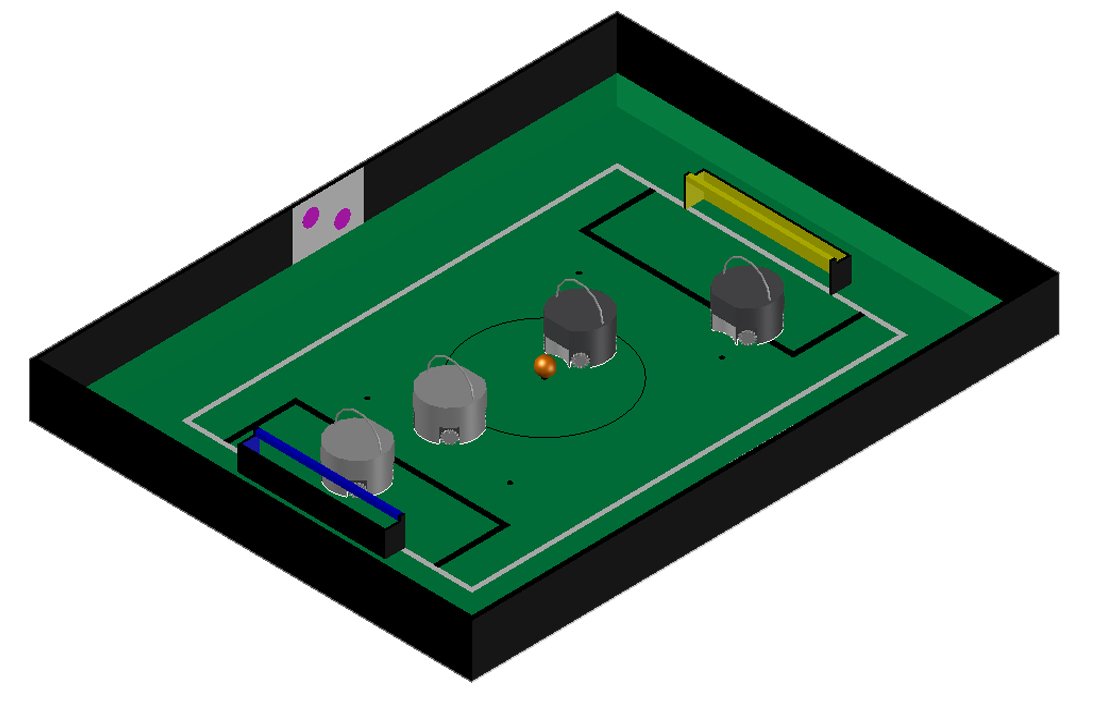
\includegraphics[width=0.7\textwidth]{media/image1_new.jpeg}
    \caption{Two teams of two robots with an orange ball on a RoboCupJunior
        Soccer field.}
    \label{fig:name}
\end{figure}

\section*{Changes from 2017 RoboCupJunior Soccer Rules}

The changes determined by the Technical Committee for this year's rules aim to
fix some organizational loopholes which have been identified in the past few
years, further standardize the playing field, bring more transparency to the
process of inspections and interviews, and bridge the gap between the Junior
and Major competitions by providing more opportunities for incorporating more
computer vision and artificial intelligence methods.

\listofchanges

\section*{Construction and Programming have to be performed exclusively by the students}

Robots must be constructed and programmed exclusively by student members of the
team. Mentors, teachers, parents or companies should not be involved in the
design, construction, assembly, programming or debugging of robots. To avoid
embarrassment and possible disqualification, it is extremely important that
teams abide by - 8.League Regulations - 8.2.3 Construction - and - 8.2.4
Programming - (found toward the end of this document) and all other
competitor's rules. If in doubt, please consult with your Regional
Representative before registering your team.

\newpage

\tableofcontents

\newpage

\section{GAMEPLAY \label{ref-001}}

\subsection{Game procedure and length of a game \label{ref-002}}

RCJ Soccer games consist of two teams of robots playing soccer against
each other. Each team has two autonomous robots. The game will consist of two
halves. The duration of each half is 10-minutes. There will be a 5-minute break
in between the halves.

The game clock will run for the duration of the halves without stopping (except
if or when a referee wants to consult another official). The game clock will be run
by a referee or a referee assistant (see Rule 7.1 for the description of a
referee assistant).

Teams are expected to be on the field 5 minutes before their game
starts. Being at the inspection table does not count in favor of this time
limit. Teams that are late for the start of the game can be penalized one goal per
30 seconds at the referee's discretion. In this (and any) situation, when the goal
differential reaches 10 the game finishes regardless of the state of the game clock.

\subsection{Pre-match meeting \label{ref-003}}

At the start of the first half of the game, a referee will toss a coin. The
team mentioned first in the draw shall call the coin. The winner of the toss
can choose either which end to kick towards, or to kick off first. The loser of the
toss chooses the other option. After the first half, teams switch sides.
The team not kicking off in the first half of the game will kick off to
begin the second half of the game.

\added[id=TC]{During the pre-match meeting the referee or their assistant may
check whether the robots are capable of playing (i.e., whether they are at
least able to follow and react to the ball). If none of the robots is capable
of playing, the game will not be played and zero goals will be awarded to both
teams.}

\subsection{Kick-off \label{ref-004}}

Each half of the game begins with a kick-off. All robots must be located on
their own side of the field. All robots must be halted. The ball is positioned
by a referee in the center of the field.

The team kicking off places their robots on the field first. Robots cannot be
placed nor remain behind the goal line or in the outer area. Robots cannot be
repositioned once they have been placed.

The team not kicking off will now place their robots on the defensive end of
the field. All robots on the team not kicking off must be at least 30 cm away
from the ball (outside of the center circle).

Robots cannot be placed behind the goal line or out of bounds.
Robots cannot be repositioned once they have been placed, except if the referee
requests to adjust their placement to make sure that the robots are placed
properly within the field positions.

On the referee's command (usually by whistle), all robots will be started
immediately by each captain. Any robots that are started early will be removed
by the referee from the field and treated as a damaged robot.

\subsection{Human interference\label{ref-005}}

Except for the kick-off, human interference from the teams (e.g. touching the
robots) during the game is not allowed unless explicitly permitted by a
referee. Violating team/team member(s) can be disqualified from the game.

The referee or a referee assistant can help robots get unstuck if the ball
is not being disputed near them and if the situation was created from normal
interaction between robots (i.e. it was not a design or programming flaw of
the robot alone). The referee or a referee assistant will pull back the robots
just enough for them to be able to move freely again.

\subsection{Ball movement \label{ref-ball-movement}}

A robot cannot hold a ball. Holding a ball is defined as taking full control
of the ball by removing all of degrees of freedom. Examples for ball holding
include fixing a ball to the robot's body, surrounding a ball using the robot's
body to prevent access by others, encircling the ball or somehow trapping the
ball with any part of the robot's body. If a ball does not roll while a robot is
moving, it is a good indication that the ball is trapped.

The only exception to holding is the use of a rotating drum (a "dribbler") that
imparts dynamic back spin on the ball to keep the ball on its surface.

Other players must be able to access the ball.

\subsection{Scoring \label{ref-007}}

A goal is scored when the ball strikes or touches the back wall of the goal.
Goals scored either by an attacking or defending robot have the same end
result: they give one goal to the team on the opposite side. After a goal, the
game will be restarted with a kick-off from the team who was scored against.
Before a kick-off, all damaged or out-of-bounds robots are allowed to return to
the playing field immediately if they are ready and fully functional.

\subsection{Goalie \label{ref-008}}

The robot moving first into the penalty area on a team's defending side
completely (with every part of it) is designated as goalie until a part of it
leaves the penalty area.

\subsection{Pushing \label{ref-pushing}}

Robots are not allowed to push each other at any time and at any place.
This applies to two robots of the same team as well as two robots of the competing opponents.
The robots may use vision, touch sensors attached to avoidance rings, or any other method
to detect the avoidance rings of other robots, see section \ref{ref-avoidance}.
A robot is allowed to play only if it can reliably detect touching or coming close to 
another robot in all directions of its own movement. When the robot detects another
robot in any particular direction, it must stop all movement in that direction immediately.
If any robot happens to push any other robot because it has failed to detect the other robot,
it is removed from play for 30 seconds by a referee.

If a goal is scored as a result of this pushed-situation, it will not be
granted.

\subsection{Pushing with ball\label{ref-pushing-with-ball}}

Robots are not allowed to push each other while both pushing the same ball in the opposite directions
even without touching each other.
Whenever the robot comes in contact with the ball, it is allowed to push it forward as long as 
there is no force working in the opposite direction. If a robot tries to push a ball forward, 
but the ball is not rolling freely, it must stop moving in the direction of the ball within 
3 seconds for at least another 3 seconds and move in another direction for at least 5 cm. 
The referee notices this by counting aloud: 1-2-3 ; 1-2-3.
Robots failing to stop pushing a stuck ball as described will be removed from the field 
for 30 seconds by the referee.
The robot is allowed to use its dribbler and back-up, or perform a side-kick in order to release 
the ball from the locked-in situation.

\subsection{Lack of progress \label{ref-lack-of-progress}}

Lack of progress occurs if there is no progress in the gameplay for a
reasonable period of time and the situation is not likely to change. Typical
lack of progress situations are when the ball is stuck between robots, when
there is no change in ball and robot's positions, or when the ball is beyond
detection or reach capability of all robots on the field.

After a visible and loud count\footnote{usually a count of five, the length of
the count could be decided by the OC before a competition as long as it's
the same length within a sub-league}, a referee will call ``lack of
progress'' and will move the ball to the nearest unoccupied neutral spot. If
this does not solve the lack of progress, the referee can move the ball to a
different neutral spot.

\subsection{Out of bounds \label{ref-011}}

If a robot's entire body moves out beyond the white line of the field, it
will be called for being out of bounds. When this situation arises, the robot
is given a one-minute penalty, and the team is asked to remove the robot from
the field. There is no time stoppage for the game itself. The robot is allowed
to return if a kickoff occurs before the penalty has elapsed.

The one-minute penalty starts when the robot is removed from play. Furthermore,
any goal scored by the penalized team while the penalized robot is on the field
will not be granted. Out-of-bounds robots can be fixed if the team needs to do
so, as described in 1.11.

After the penalty time has passed, robot will be placed on the unoccupied
neutral spot nearest to where it has been taken off, \replaced[id=TC]{and not
directly aiming towards the ball}{orientated towards the nearest wall}.
\added[id=TC]{Alternatively, the referee may instruct the
team to place the robot on the neutral spot on the side of the field
currently farthest from the ball, oriented towards the closest wall. }

A referee can waive the penalty if the robot was accidentally pushed out of
bounds by \replaced[id=TC]{an opposing}{any other} robot. In such a case, the
referee may have to slightly push the robot back onto the field.

The ball can leave and bounce back into the playing field. The referee calls
``out of reach'', and will move the ball to the nearest unoccupied neutral spot
when one of the following condition occurs:

\begin{enumerate}
    \item the ball remains outside the playing field too long,
        after a visible and loud count, (usually a count of five, the length of
        the count can be decided by the OC before a competition as long as it
        is the same length within a sub-league)

    \item any of the robots are unable to return it into the playing field
        (without their whole body leaving the playing field), or

    \item the referee determines that the ball will not come back into the
        playing field.

\end{enumerate}

\subsection{Damaged robots \label{ref-012}}

If a robot is damaged, it has to be taken off the field and must be fixed
before it can play again. Even if repaired, the robot must remain off the field
for at least one minute or until the next kickoff is due. If all robots have
moved out of bounds, the penalties are discarded and the match resumes with a
neutral kickoff.

Some examples of a damaged robot include:

\begin{itemize}

\item it does not respond to the ball, or is unable to move (it lost pieces,
    power, etc.).

\item it continually moves into the goal or out of the playing field.

\item it turns over on its own accord.

\end{itemize}

Computers and repair equipment are not permitted in the playing area during
gameplay. Usually, a team member will need to take the damaged robot to an
``approved repair table'' near the playing area.\deleted[id=TC]{, located
inside the competitors working area.} A referee may permit robot sensor
calibration, computers and other tools in the playing area, only for the 5
minutes before the start of each half. \added[id=TC]{Reprogramming of robots
during the gameplay can only happen when they are out of game (i.e., damaged
or out of bounds), or when explicitly allowed by the referee.}

After a robot has been fixed, it will be placed on the unoccupied neutral spot
nearest to where it has been taken off, \replaced[id=TC]{and not directly aiming
towards the ball}{orientated towards the nearest wall}.
\added[id=TC]{Alternatively, the referee may instruct the team to place
the robot on the neutral spot on the side of the field currently farthest from
the ball, orientated towards the nearest wall.}
A robot can only be returned to the field if the damage has been
repaired. If the referee notices that the robot was returned to the field with
the same original problem, s/he may ask the robot to be removed, and proceed
with the game as if the robot had not been returned.

\textbf{Only the referee decides whether a robot is damaged.} A robot can only
be taken off or returned with the referee's permission.

\replaced[id=TC]
{
If both robots from the same team are deemed damaged at kickoff,
gameplay will be paused and the remaining team will be awarded 1 goal for
each elapsed 30 seconds that their opponent's robots remain damaged.
}
{
If both robots from the same team are deemed damaged during gameplay, the clock
continues and the remaining team gets one initial goal and rests while waiting
for the opponent's return to play. The remaining team will also get one
additional goal for each elapsed 30 seconds the opponent's robots remain
damaged. Once a 10 goal difference occurs or the remaining time finishes, the
team with no functional robots forfeits the game.
}

However, these rules only apply when none of the two robots from the same team
were damaged as the result of the opponent team violating the rules.

\subsection{Multiple defense \label{ref-013}}

Multiple defense occurs if more than one robot from the defending team enters
its penalty area with some part and substantially affects the game. The robot
farther from the ball will be moved to the nearest neutral spot.
\added[id=TC]{Only} the referee can take this action at any time when both
robots linger in their penalty area.

\added[id=TC]{If multiple defense happens repeatedly in a short amount of time,
the offending robot will be moved to an unoccupied neutral spot on the other
side of the field, orientated towards the nearest wall.}
\replaced[id=TC]{If any robot needs to be moved to an unoccupied neutral spot
more than \textbf{three times} during its single uninterrupted time chunk on the
field, it}{If multiple defense happens repeatedly, the robot}
will be deemed damaged\footnote{For the purpose of this rule a time chunk is
defined as time between two events when the robot is taken off the field for
some reason (e.g. at the end of the first half of the game, when it is deemed
damaged or out of bounds).}.

\subsection{Interruption of Game \label{ref-interruption}}

In principle, a game will not be stopped.

A referee can stop the game if there is a situation on or around the field
which the referee wants to discuss with an official of the tournament or if the
ball malfunctions and a replacement is not readily available.

When the referee has stopped the game, all robots must be stopped and remain on
the field untouched. The referee may decide whether the game will be
continued/resumed from the situation in which the game was stopped or by a
kick-off.

\section{TEAM \label{ref-015}}

\subsection{Regulations \label{ref-team-regulations}}

A team must have more than one member to form a RoboCupJunior team to
participate in the International event. A team member(s) and/or robot(s) cannot
be shared between teams.

Each team member needs to carry a technical role.

Each team must have a \textbf{captain}. The captain is the person responsible
for communication with referees. The team can replace its captain during the
competition. Team is allowed to have \added[id=TC]{at most two} members beside
the field during game play: they will usually be the captain and an assistant
team member.

\subsection{Violations \label{ref-violations}}

Teams that do not abide by the rules are not allowed to participate.

Any person close to the playing field is not allowed to wear any orange, yellow
or blue clothes that can be seen by the robots (to avoid interference). A
referee can require a team member to change clothes or to be replaced by
another team member if interference is suspected.

The referee can interrupt a game in progress if any kind of interference from
spectators is suspected (color clothing, IR emitters, camera flashes, mobile
phones, radios, computers, etc.).

This needs to be proved to an OC member if a claim is placed by the other team.
A team claiming that their robot is affected by colors has to show the
proof/evidence of the interference.

\begin{figure}[H]
    \centering
    
\includegraphics[width=0.4\textwidth]{media/image2.png}
    \caption{Persons close to the playing field are not allowed to wear orange,
        yellow or blue clothes}
    \label{fig:spectators}
\end{figure}


\section{ROBOTS\label{ref-018}}

\subsection{ Number of robots / substitution \label{ref-number-of-robots}}

Each team is allowed to have at most two robots for the full tournament. The
substitution of robots during the competition within the team or with other
teams is forbidden.

\subsection{ Interference \label{ref-interference}}

Robots are not allowed to be colored orange, yellow, blue, or any other color
that can be confused with a landmark (see 4.3) in order to avoid interference.
Orange, yellow, blue or any landmark-like colored parts used in the
construction of the robot must either be occluded by other parts from the
perception by other robots or be taped/painted with a neutral color.

The robot must not emit infrared light. However, optical sensors (e.g.
infrared-distance-sensors) may be used as long as they do not affect other
robots. This needs to be proved by a referee or an OC member if a claim is
placed by the other team.

Infrared light reflecting materials must not be used on the outside. If robots
are painted, they must be painted matte. Minor parts that reflect infrared
light could be used as long as other robots are not affected. A team claiming
that their robot is affected by the other team's robot reflecting infrared
light must show the proof/evidence of the interference.

Robots must not produce magnetic interference in other robots on the field.
This needs to be proved by a referee or an OC member if a claim is placed by
the other team.

\subsection{ Control \label{ref-control}}

The use of remote control of any kind is not allowed during the match. Robots
must be started and stopped manually by humans and be controlled autonomously.

\subsection{ Communication \label{ref-022}}

Robots are not allowed to use any kind of communication during game play unless
the communication between two robots is via Bluetooth class 2 or class
3\footnote{range shorter than 20 meters} or via any other device that
communicates using the 802.15.4 protocol (e.g., ZigBee and XBee). Teams are
responsible for their communication. The availability of frequencies cannot be
guaranteed.

\subsection{Agility \label{ref-agility}}

Robots must be constructed and programmed in a way that their movement is not
limited to only one dimension (defined as a single axis, such as). They must move in all
directions, for example by turning. Robots must respond to the ball in a direct
forward movement. For example, it is not enough to basically just move left and
right in front of their own goal, it must also move directly towards the ball in
a forward movement. At least one team robot must be able to seek and approach
the ball anywhere on the field, unless the team has only one robot on the field
at that time. \added[id=TC]{Goalie has to approach the ball in the whole
penalty area.}

Robots must be constructed \deleted[id=TC]{or programmed }in a way that they do
not enter the goal. Robots are allowed to use the cross-bar in order to avoid
entering the goal. This rule applies to all robots on the field. Any robot
that moves into the goal 3 times during a period of 20 seconds is deemed to be
damaged (see \hyperref[ref-012]{1.11}).

\begin{figure}[H]
    \centering
    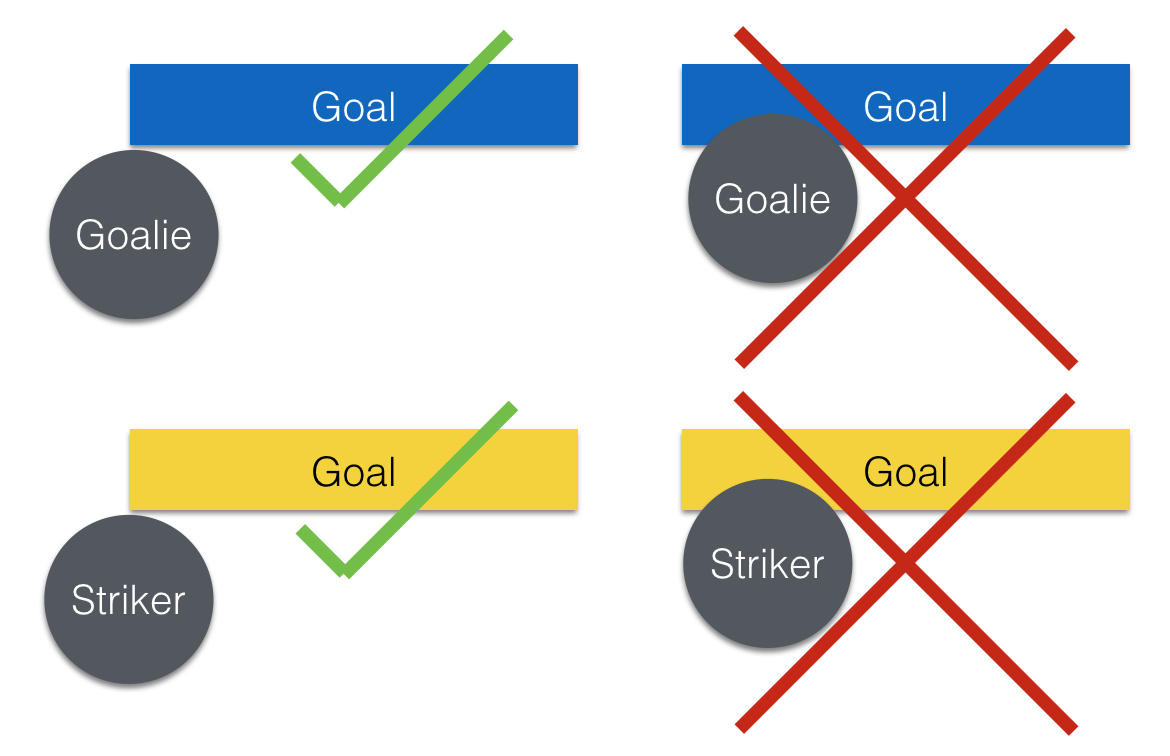
\includegraphics[width=0.8\textwidth]{media/image3.png}
    \caption{Acceptable and unacceptable position of Goalie and Striker}
    \label{fig:robot_in_goal}
\end{figure}

\subsection{ Avoidance \label{ref-avoidance}}

In order to be able to detect each other reliably, all robots must have 
an avoidance ring. The avoidance ring is a 2.54 cm high hollow cylinder surrounding
the robot. When viewed from top, this cylinder forms a convex hull of the robot shape.
It is installed at the height of 12 cm  - 14.54 cm from the field floor.
Its color must be the same as the color of the ball.
See also section \ref{ref-pushing}.

\subsection{ Handle \label{ref-handle}}

All robots must have a stable handle to hold and to lift them. The handle must
be easily accessible, for example on top of the robot. The dimensions of the
handle may exceed the 22 cm height limitation, but the part of the handle that
exceeds this 22 cm limit cannot be used to mount components of the robot.

\subsection{ Top Markers\label{ref-top-markers}}

A robot must have markings in order to be distinguished by the referee. Each
robot must have a white plastic circle with a diameter of at least 4 cm mounted
horizontally on top. This white circle will be used by the referee to write
numbers on the robots using markers, therefore the white circles must be
accessible and visible.

Before the game, the referee will designate the numbers for each robot and will
write them on the top white circle. Robots not carrying the top white circle
are not eligible to play.

\begin{figure}[H]
    \centering
    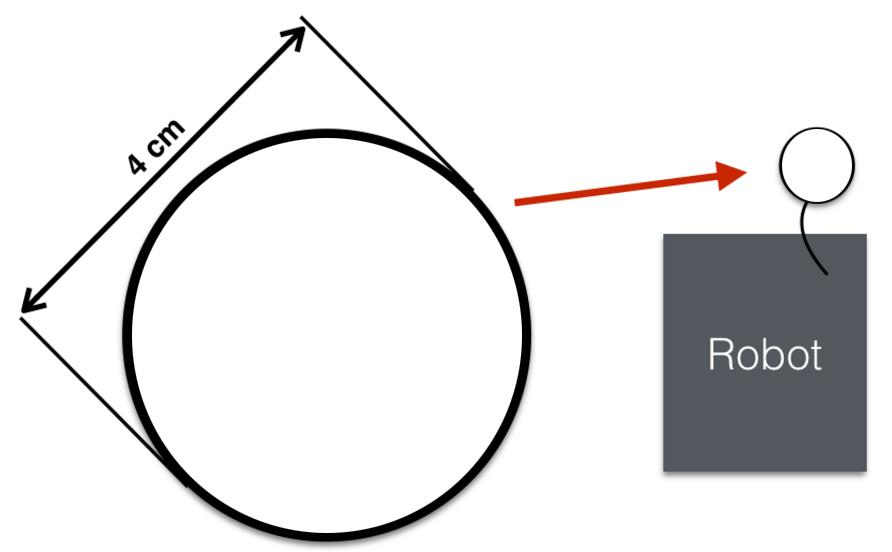
\includegraphics[width=0.5\textwidth]{media/image4.jpeg}
    \caption{A visualization of the top marker}
    \label{fig:top_marker}
\end{figure}

\subsection{ Additional regulations of the sub-leagues \label{ref-sub-leagues}}

A tournament may be organized in different sub-leagues. Each sub-league (e.g.
``Soccer Open'' and ``Soccer Lightweight'') has its own additional regulations,
including regulations affecting the construction of robots. They are outlined
in section \textbf{8. League Regulations}.

\subsection{ Violations \label{ref-027}}

Robots that do not abide by the specifications/regulations (see 8. League
Regulations for more details) are not allowed to play, unless these rules
specify otherwise. If violations are detected during a running game the team is
disqualified for that game. If similar violations occur repeatedly, the team
can be disqualified from the tournament.

\section{FIELD \label{ref-028}}

\subsection{Kind of field \label{ref-029}}

There is only one kind of field for all sub-leagues.

\subsection{ Dimensions of the field \label{ref-030}}

The playing-field is 122 cm by 183 cm. The field is marked by a white line
which is part of the playing-field. Around the playing-field, beyond the white
line, is an outer area of 30 cm width. The floor near the exterior wall
includes a wedge, which is an incline with a 10 cm base and 2 cm rise for
allowing the ball to roll back into play when it leaves the playing field.
Total dimensions of the field, including the outer area, are 182 cm by 243 cm.
It is recommended that the field be positioned 70 to 90 cm off the ground.

\subsection{ Walls \label{ref-walls}}

Walls are placed all around the field, including behind the goals and the
out-area. The height of the walls is 22 cm. The walls are painted matte black.

There are colored landmarks positioned on each wall. \added[id=TC]{They consist
of two magenta circles printed on letter paper (A4, 210mm x 297mm). They
measure 70mm in diameter and their centers are 150mm apart from each other.
Their position within the landmark as well as the position of the
respective landmarks on the field can be seen in Figure
\ref{fig:landmarks_blueprint}. Note that these landmarks are always positioned
in the middle of the wall.}.

\begin{figure}[H]
    \centering
    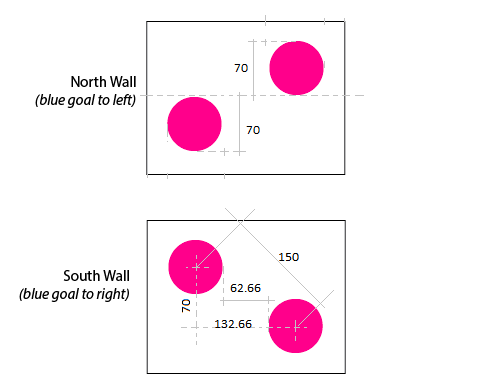
\includegraphics[width=0.7\textwidth]{media/landmarks_blueprint.png}
    \caption{Position of magenta circles on each of the two landmarks, as well
        as the position of each of the two landmarks on the field. Note that in
        this case ''blue goal to the left/right'' here to the situation when
        one is looking directly at the blue goal from the center of the field.
        For more information on the position of landmarks please consult the
        Field diagrams section.}
    \label{fig:landmarks_blueprint}
\end{figure}

\added[id=TC]{The color used for these landmarks (magenta) is defined (for the
    purpose of this section) to be one of the following:}

\begin{itemize}
    \item \texttt{RGB (217, 1, 2)}
    \item \texttt{CMYK (0, 255, 0, 0)}
    \item PANTONE Process Magenta C (\url{https://www.pantone.com/color-finder/Process-Magenta-C})
\end{itemize}

\subsection{ Goals \label{ref-032}}

The field has two goals, centered on each of the shorter sides of the playing
field. The goal inner space is 60 cm width, 10 cm high and 74 mm deep, box
shaped. It has a cross-bar on top (to prevent robots from entering the goal and
to allow checking if the ball scored). The height of the cross-bar is 2 cm. The
goal ``posts'' are positioned over the white line marking the limits of the
field. The cross-bar is exactly over the white line. The interior walls and the
cross-bar of each goal are painted, one goal yellow, the other goal blue. The
exterior (including the goal post and frame) are painted black (see the field
diagrams).

\subsection{ Floor \label{ref-033}}

The floor consists of dark green carpet on top of a hard level surface.
\deleted[id=TC]{The carpet should be of a quality that will resist the wear and
tear of spinning wheels.} All straight lines on the field should be painted and
have a width of 20 mm.

\subsection{ Neutral spots \label{ref-034}}

There are five neutral spots defined in the field. One is in the center of the
field. The other four are adjacent to each corner, located 45 cm along the long
edge of the field, aligned with each goal post towards the middle of the field
(from the goal post). The neutral spots can be drawn with a thin black marker.
The neutral spots ought to be of circular shape measuring 1 cm in diameter.

\subsection{ Center circle \label{ref-035}}

A center circle will be drawn on the field. It is 60 cm in diameter. It is a
thin black marker line. It is there for Referees and Captains as guidance
during kick-off.

\subsection{ Penalty areas \label{ref-036}}

In front of each goal there is a 30 cm wide and 90 cm long penalty area.

The penalty areas are marked by a black line of 20 mm width. The line is part
of the area.

A robot is considered inside the Penalty Area when it is completely inside.

\subsection{Lighting and Magnetic Conditions \label{ref-lighting-conditions}}

The fields should be placed in a way that the influence by external infrared
light is as low as possible and that the magnetic field of the earth is
disturbed as little as possible. Perfect conditions cannot be guaranteed,
however. Teams must come to tournaments being prepared to calibrate their
robots based on the lighting and magnetic conditions at the venue.

\section{BALL \label{section:ball}}

\subsection{Specification for Soccer Lightweight Ball \label{ref-sec-spec-plused}}

See Appendix \ref{ref-pulsed-spec} (Technical Specification for pulsed Soccer
Ball).

\subsection{Specification for Soccer Open Ball\label{ref-sec-spec-open}}

See Appendix \ref{ref-passive-spec} (Technical Specification for passive Soccer
Ball).

\subsection{ Tournament balls \label{ref-tournament-balls}}

Balls for the tournament must be made available by the organizers. Organizers
are not responsible for providing balls for practice.

\section{CODE OF CONDUCT\label{ref-code-of-conduct}}

\subsection{ Fair Play \label{ref-041}}

It is expected that the aim of all teams is to play a fair and clean game of
robot soccer. It is expected that all robots will be built with consideration
to other participants.

Robots are not allowed to cause deliberate interference with or damage to other
robots during normal game play.

Robots are not allowed to cause damage to the field or to the ball during
normal game play.

\added[id=TC]{A robot that causes damage may be disqualified from a specific
match at the referee's discretion. The OC will also be informed.}

Humans are not allowed to cause deliberate interference with robots or damage
to the field or the ball.

\subsection{ Behavior \label{ref-042}}

All participants are expected to behave themselves. All movement and behavior
is to be of a subdued nature within the tournament venue.

\subsection{ Help \label{ref-043}}

Mentors (teachers, parents, chaperones, and other adult team-members including
translators) are not allowed in the student work area unless it is explicitly
but temporarily permitted by a member of the Organizing Committee. Only
participating students are allowed to be inside the work area.

Mentors must not touch, build, repair, or program any robots.

\subsection{ Sharing \label{ref-044}}

The understanding that any technological and curricular developments should be
shared among the RoboCup and RoboCupJunior participants after the tournament
has been a part of world RoboCup competitions.

\subsection{ Spirit \label{ref-045}}

It is expected that all participants, students, mentors, and parents will
respect the RoboCupJunior mission. \textbf{\textit{It is not whether you win or
lose, but how much you learn that counts!}}

\subsection{ Violations / Disqualification \label{ref-046}}

Teams that violate the code of conduct can be disqualified from the tournament.
It is also possible to disqualify only single person or single robot from
further participation in the tournament.

In less severe cases of violations of the code of conduct, a team will be given
a warning by showing it a yellow card. In severe or repeated cases of
violations of the code of conduct a team can be disqualified immediately
without a warning by showing it the red card.

\section{CONFLICT RESOLUTION \label{ref-conflict-resolution}}

\subsection{Referee and referee assistant \label{ref-048}}

The referee is a person in charge of making decisions with regards to the game,
according to these rules, and may be assisted by a referee assistant.

\textbf{During gameplay, the decisions made by the referee and/or the referee assistant are final.}

Any argument with the referee or the referee assistant can result in a warning.
If the argument continues or another argument occurs, this may result in
immediate disqualification from the game.

\added[id=TC]{Only the captain has a mandate to freely speak to the referee
and/or their assistant. Shouting at a referee and/or their assistant, as well
as demanding a change in ruling can be directly penalized by a warning at
the referee's discretion.}

At the conclusion of the game, the result recorded in the scoresheet is final.
The referee will ask the captains to add written comments to the scoresheet if
they consider them necessary. These comments will be reviewed by the OC
members.

\subsection{Rule clarification \label{ref-049}}

Rule clarification may be made by members of the RoboCupJunior Soccer Technical
Committee and Organizing Committee, if necessary even during a tournament.

\subsection{Rule modification \label{ref-050}}

If special circumstances, such as unforeseen problems or capabilities of a
robot occur, rules may be modified by the RoboCupJunior Soccer Organizing
Committee Chair in conjunction with available Technical Committee and
Organizing Committee members, if necessary even during a tournament.

\subsection{Regulatory statutes \label{ref-051}}

Each RoboCupJunior competition may have its own regulatory statutes to define
the procedure of the tournament (for example the SuperTeam system, game modes,
the inspection of robots, interviews, schedules, etc.). Regulatory statutes
become a part of this rule.

\section*{FIELD DIAGRAMS}

\begin{center}

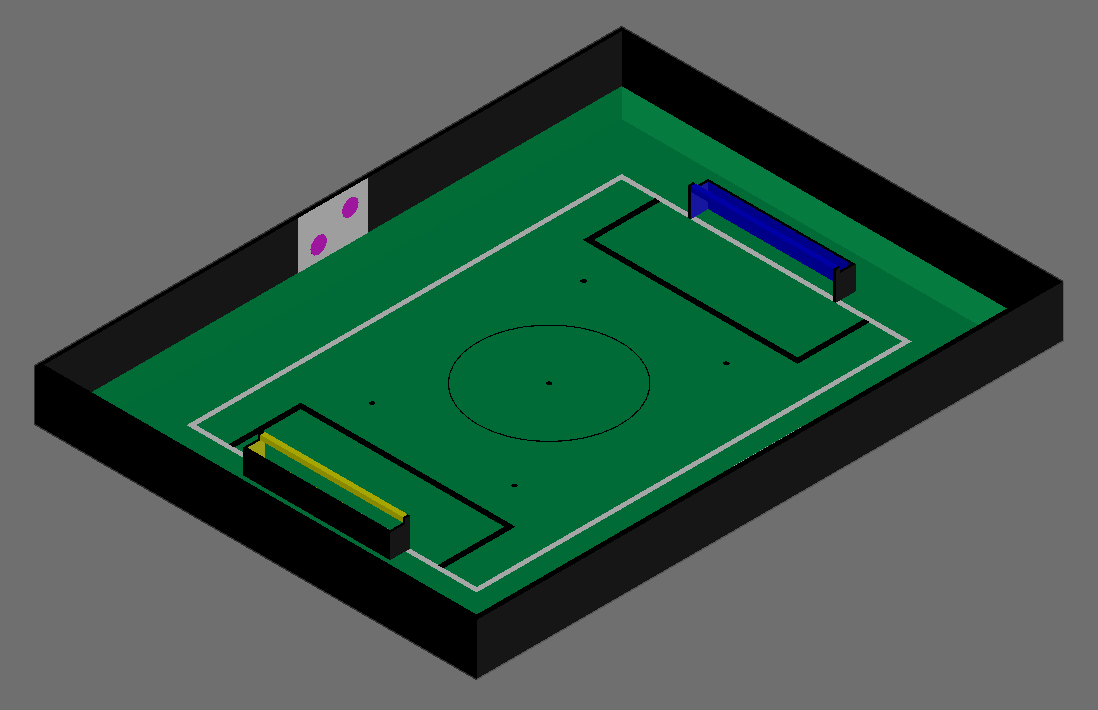
\includegraphics[width=0.9\textwidth]{media/image5_new.jpeg}

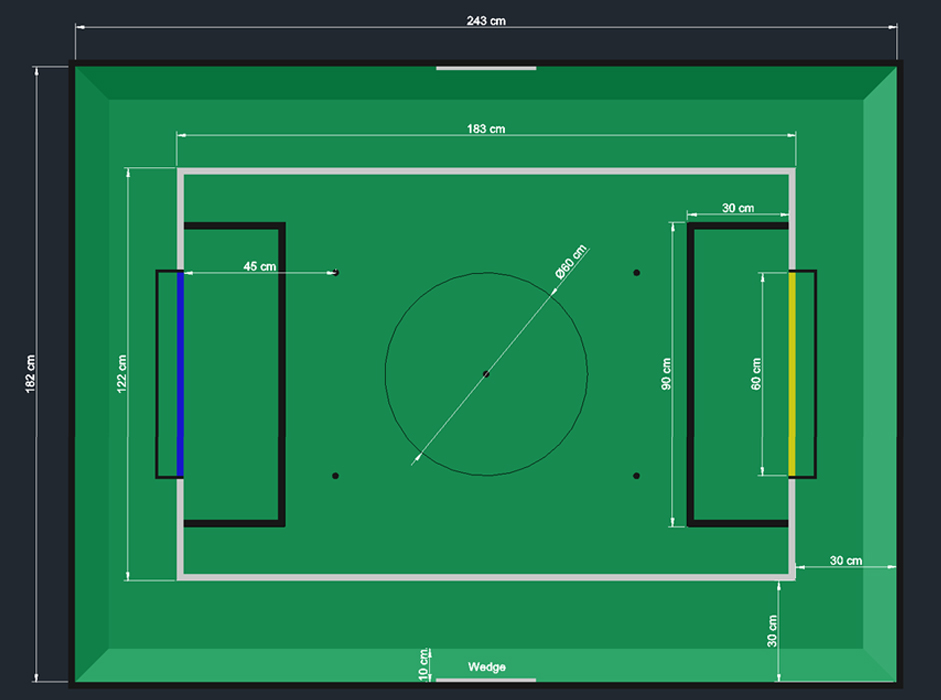
\includegraphics[width=0.9\textwidth]{media/image6_new.jpeg}

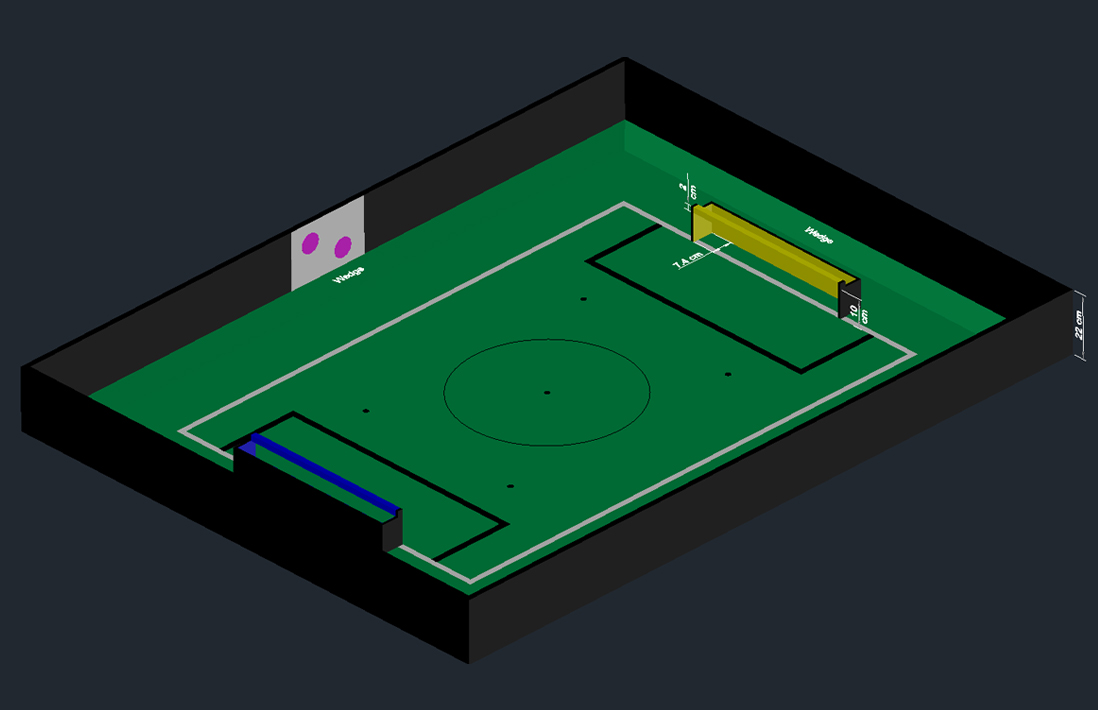
\includegraphics[width=0.8\textwidth]{media/image7_new.jpeg}

\end{center}

\section{LEAGUE REGULATIONS \label{section:league_regulations}}

\subsection{ Preamble \label{ref-053}}

According to rule 3.8 of the RoboCupJunior Soccer Rules, each league has its
own additional regulations. They become a part of the rules.

For RoboCupJunior 2018, there are two sub-leagues as follows
\footnote{biggest differences are described in 8.2.1 Dimensions}:

\begin{itemize}

\item Soccer Lightweight.

\item Soccer Open.

\end{itemize}

\added[id=TC]{All team members between 12 and 19 years old on July 1st, 2018}.

As described in sections 5.1 and 5.2, the matches in the Soccer Open sub-league
are conducted using a passive ball, whereas the matches in the Soccer
Lightweight sub-league are played using the IR ball.

\subsection{Regulations \label{ref-054}}

\subsubsection{Dimensions \label{ref-055}}

Robots will be measured in an upright position with all parts extended. A
robot's dimensions must not exceed the following limits:

\begin{table}
\begin{tabularx}{\textwidth}{
p{\dimexpr 0.33\linewidth-2\tabcolsep}
p{\dimexpr 0.33\linewidth-2\tabcolsep}
p{\dimexpr 0.33\linewidth-2\tabcolsep}}
sub-league & \textbf{Soccer} \textbf{Open} & \textbf{Soccer Lightweight} \\
size / diameter & \O{} 22.0 cm & \O{} 22.0 cm \\
height & 22.0 cm * & 22.0 cm * \\
weight & 2400 g ** & 1100 g ** \\
ball-capturing zone & 2.5 cm & 3.0 cm \\
voltage & 15.0 V\textcolor{red}{***} & 12.0 V\textcolor{red}{***} \\

\end{tabularx}

\end{table}

* The handle and the top markers of a robot may exceed the height.

** The weight of the robot includes that of the handle.

*** We encourage teams to include protection circuits for Lithium-based
batteries

*** Voltage limits relate to the \textbf{nominal values}, deviations at the power pack
due to the fact that charged will be tolerated.

Ball-capturing zone is defined as any internal space created when a straight
edge is placed on the protruding points of a robot. This means the ball must
not enter the concave hull of a robot by more than the specified depth.
Furthermore, it must be possible for another robot to take possession of the
ball.

\subsubsection{Limitations\label{ref-056}}

A single robot can only use one camera. All commercial omnidirectional
lenses/cameras are not permitted. Only omnidirectional lenses/cameras made by
students are permitted, meaning that their construction needs to be primarily
and substantially the original work of a team. Teams using them on their robots
must prove how they made them on their presentation poster and at an interview.
For the purpose of these rules omnidirectional is defined as having a
field-of-view of more than 140 degrees horizontally and more than 80 degrees
vertically (these values reflect the optical system of the human eye).

Voltage pump circuits are permitted only for a kicker drive. All other
electrical circuits inside the robot cannot exceed 15.0 V for Soccer Open and
12.0 V for Soccer Lightweight. Each robot must be designed to allow verifying
the voltage of power packs and its circuits, unless the nominal voltage is
obvious by looking at the robot, its power packs and connections.

Pneumatic devices are allowed to use ambient air only.

Kicker strength is subject to compliance check at any time during the
competition. During gameplay, a referee can ask to see a sample kick on the
field before each half, when a damaged robot is returned to the field, or when
the game is about to be restarted after a goal. If the referee strongly
suspects that a kicker exceeds the power limit, he can require an official
measurement with the 'Kicker Power Measure Device'. (See the Appendix III:
Kicker Power Measure Device' for details.)

\subsubsection{Construction \label{ref-057}}

Robots must be constructed exclusively by the student members of a team.
Mentors, teachers, parents or companies may not be involved in the design,
construction, and assembly of robots.

For the construction of a robot, any robot kit or building block may be used as
long as the design and construction are primarily and substantially the
original work of a team. This means that commercial kits may be used but must
be substantially modified by the team. It is neither allowed to mainly follow a
construction manual, nor to just change unimportant parts.

Indications for violations are the use of commercial kits that can basically
only be assembled in one way or the fact that robots from different team(s),
build from the same commercial kit, all basically look or function the same.

Robots must be constructed in a way that they can be started by the captain
without the help of another person.

Since a contact with an opponent robot and/or dribbler that might damage some
parts of robots cannot be fully anticipated, robots must have all its active
elements properly protected with resistant materials. For example, electrical
circuits and pneumatic devices, such as pipelines and bottles, must be
protected from all human contact and direct contact with other robots. When
batteries are transported or moved, it is recommended that safety bags be used.
Reasonable efforts should be made to make sure that in all circumstances robots
avoid short-circuits and chemical or air leaks.

\subsubsection{Programming \label{ref-058}}

Robots must be programmed exclusively by student members of the team. Mentors,
teachers, parents or companies should not be involved in the programming and
debugging of robots.

For the programming of the robots, any programming language, interface or
integrated development environment (IDE) may be used. The use of programs that
come together with a commercial kit (especially sample programs or presets) or
substantial parts of such programs are not allowed. It is not allowed to use
sample programs, not even if they are modified.

\subsubsection{Inspections \label{ref-059}}

Robots must be inspected and certified every day before the first game is
played. The Organizing Committee may request other inspections if necessary,
including random inspections which may happen at any time. The routine
inspections include:

\begin{itemize}
\item Weight restrictions for the particular sub-league (see 8.2.1).

\item Robot dimensions (see 8.2.1).

\item Voltage restrictions (see 8.2.1 and 8.2.2).

\item Kicker strength limits, if the robot has a kicker. (See the Appendix III: Kicker Power Check Device.)
\end{itemize}

Proof must be provided by each team that its robots comply with these
regulations, for example, by a detailed documentation or log book. Teams may be
interviewed about their robots and the development process at any time during a
tournament.

See an example of the inspection sheet that members of the OC will use in
Appendix V - Inspections Sheet Example. Note that the sheet will be updated by
OC members before the competition to match this year's rules, but the important
aspects which are checked will stay the same.


\newpage

\section{International Competition}

\subsection{Team}

\replaced[id=TC]{Maximum team size is 4 members for RoboCupJunior 2018.}{Maximum team size is 5 members for RoboCupJunior 2017.}

Starting in 2017, Soccer Lightweight team members can participate in the World
Championship only twice. After their second participation, they need to move to
Soccer Open. Note that counting starts with the 2017 World Championship.

\subsection{Interviews \label{ref-060}}

During the international competition, the Organizing Committee will arrange to
interview teams during the Setup Day of the event. This means that the teams
need to be already present early on this day. Teams must bring robots, the code
that is used to program them and any documentation to the interview.

During an interview, at least one member from each team must be able to explain
particularities about the team's robots, especially with regards to its
construction and its programming. An interviewer may ask the team for a
demonstration. The interviewer may also ask the team to write a simple program
during the interview to verify that the team is able to program its robot.

All teams are expected to be able to conduct the interview in English. If this
poses a problem, the team may ask for a translator to be present at the
interview. If the OC is not able to provide a translator, the team is required
to do so. During the interview, the team will be evaluated using so called
Rubrics, which are published on the website mentioned in the beginning of these
rules.

The Technical Committee recommends the implementation of interviews in regional
competitions as well, but this is not mandatory.

\subsection{\added[id=TC]{Technical Challenges}}

\textcolor{red}{Inspired by the major leagues and the need for further technological
advancement of the leagues, the Technical Committee has decided to introduce so
called ``Technical Challenges''.}

\textcolor{red}{The idea of these challenges is to give the teams an opportunity to show off
various abilities of their robots which may not get noticed during the regular
games. Furthermore, the Technical Committee envisions these challenges to be a
place for testing new ideas that may make it to the future rules, or otherwise
shape the competition.}

\textcolor{red}{Any RoboCupJunior Soccer team will be eligible to try to tackle these
challenges. Unless otherwise stated, any robot taking part in these
challenges needs to abide by these rules in order to successfully complete it.}

\subsubsection{\added[id=TC]{Precision shooter}}

\textcolor{red}{\textit{The results in soccer are evaluated by the number of
scored goals. History usually does not care how they were scored. For
the spectators, however, this usually makes all the difference.}}

\textcolor{red}{This challenge consists of six rounds. In each round, the robot
starts from its own penalty area oriented towards the goal. The ball is
placed randomly (by rolling a die) inside this half of the field on one of
the following spots:}

\begin{enumerate}
    \item \textcolor{red}{Left neutral spot}
    \item \textcolor{red}{Right neutral spot}
    \item \textcolor{red}{Left corner of the penalty area}
    \item \textcolor{red}{Right corner of the penalty area}
    \item \textcolor{red}{Left corner of the field}
    \item \textcolor{red}{Right corner of the field}
\end{enumerate}

\textcolor{red}{The robot needs to locate the ball and score a goal while
staying on its own half of the field. Each round takes at most 20 seconds.}

\begin{itemize}
    \item \textcolor{red}{The team is free to pick which side to kick from.}
    \item \textcolor{red}{The same robot must  be used for all rounds.}
    \item \textcolor{red}{The robot must stay on its half of the field for the
            goal to count, but ''out of bounds'' rules do not apply.}
\end{itemize}

\textcolor{red}{Initially, the opposite goal is completely open (see Figure
\ref{fig:goal_parts}). After each
scored goal a member of the team rolls a die and the part of the goal that
corresponds to the number on the dice will be covered with a black box. If
this part of the goal is already covered, the die will be rolled again (see
Figure \ref{fig:goal_parts_filled}).}

\textcolor{red}{The result of this challenge is the number of scored goals.}

\begin{figure}
  \centering
  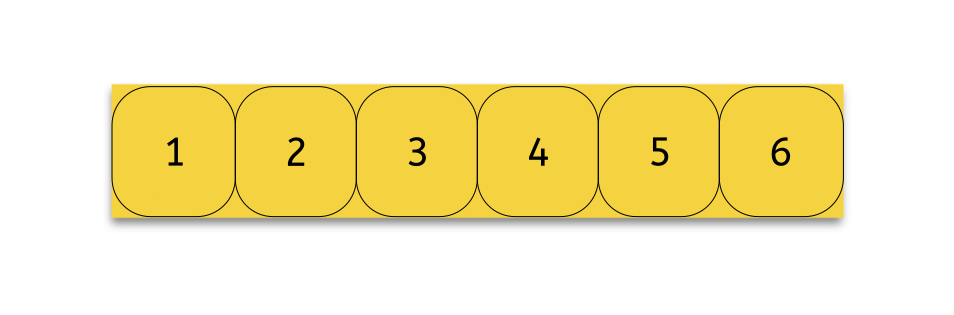
\includegraphics[width=.9\linewidth]{media/goal_parts}
  \caption{Partitioning of the goal into 6 parts.}
  \label{fig:goal_parts}
\end{figure}%
\begin{figure}
  \centering
  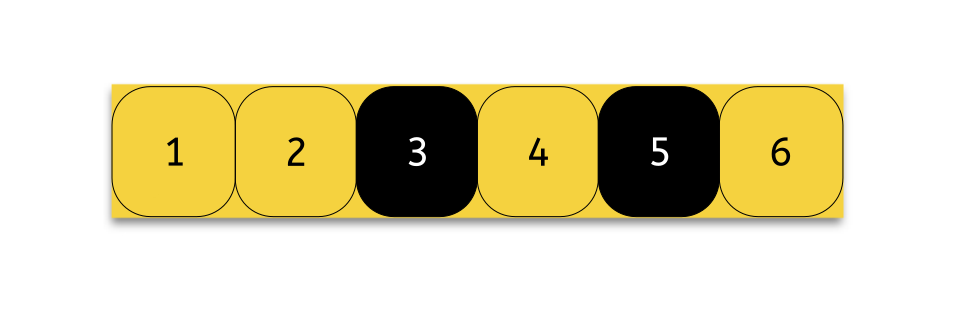
\includegraphics[width=.9\linewidth]{media/goal_parts_filled}
  \caption{State of the goal after two rounds, where the number 3 and number 5
      were rolled on a die after each round and the respective parts of the
      goal are covered. Note that if number 3 or 5 will get rolled in the next
      rounds, a new roll of a die will follow.}
  \label{fig:goal_parts_filled}
\end{figure}

\subsubsection{\added[id=TC]{Landmark localization}}

\textcolor{red}{\textit{With the inclusion of landmarks on the field, the
question of “where am I” that each soccer robot normally asks itself is
one that can be answered in a pretty simple manner.}}

\textcolor{red}{In this challenge the robot is tasked with visiting the
    following points of interest on the field that includes the 2017 version of
    landmarks:}

\begin{enumerate}
    \item \textcolor{red}{Yellow goal}
    \item \textcolor{red}{Cyan landmark}
    \item \textcolor{red}{Cyan-red landmark}
    \item \textcolor{red}{Red landmark}
    \item \textcolor{red}{Blue goal}
    \item \textcolor{red}{Green landmark}
    \item \textcolor{red}{Green-magenta landmark}
    \item \textcolor{red}{Magenta landmark}
\end{enumerate}

\textcolor{red}{A point of interest is considered visited when a part of the
    robot is located in a 10cm radius from a given point of interest.
    Furthermore, the robot is required to signal that it visited a given
    landmark in some way (visually, audibly, or in any other way that can be
    easily distinguished from normal operation by a referee).}

\textcolor{red}{While the order of points of interests mentioned above stays
    fixed, before each start of the challenge their position on the field will
    be randomly changed.}

\textcolor{red}{The result of this challenge is the number of points of
    interests visited in correct order.}

\subsubsection{\added[id=TC]{Innovative usage of landmarks}}

\textcolor{red}{The six landmarks on the field were introduced in the previous
    version of the rules in an attempt to provide more opportunities for
    experimentation with localization on the field. However, the change has
    shown to be quite disruptive (in many cases it caused more harm than good)
    and so a new version of landmarks has been designed for this year in order
    to fix this.}

\textcolor{red}{Since these landmarks have been in the rules for quite some
    time now and some teams may have invested into using them, this challenge
    has been designed to give them an opportunity to present their work and
    receive some bonus points for it as well.}

\textcolor{red}{The result of this challenge is a binary decision: a set of
    bonus points awarded to a team which manages to persuade the OC that they
    use the landmarks in an innovative way.}

\subsection{Further information on International Competition \label{ref-061}}

All teams qualified to the international competition \textbf{must} share their
designs, both hardware and software, with all present and future participants.
These teams are also required to send a digital portfolio before the
competition. Further details on how will be provided by the Organizational
Committee.

During the competition days of the International Competition (as well as before
the event) the team members are responsible for checking all relevant
information published by the Soccer Organizational Committee, General Chairs,
or any other RoboCup official.

Teams competing in the International Competition can receive awards for their
performance. These awards are decided and introduced by the Organizational
Committee, which publishes all necessary details well before the actual event.
In the past years they were awarded for best poster, presentation, robot
design, team spirit and individual games. Note that as stated in rule 6.5
``\textbf{\textit{\textcolor{red}{It is not whether you win or lose, but how
much you learn that counts!''.}}}

\appendix
\section{Technical Specification for pulsed Soccer Ball\label{ref-pulsed-spec}}

\subsection{Preamble}

Answering to the request for a soccer ball for RCJ tournaments that would be
more robust to interfering lights, less energy consuming and mechanically more
resistant, the RCJ Soccer Technical Committee defined the following technical
specifications with the special collaboration from EK Japan and HiTechnic.

Producers of these balls must apply for a certification process upon which they
can exhibit the RCJ-compliant label and their balls used in RCJ tournaments.

Balls with these specifications can be detected using specific sensors from
HiTechnic (IRSeeker - information on distance and angle) but also common IR
remote control receivers (TSOP1140, TSOP31140, GP1UX511QS, ... - on-off
detection with a possible gross indication of distance).

\subsection{I.2. Specifications}

\subsubsection{IR light}

The ball emits infra-red (IR) light of wavelengths in the range 920nm - 960nm,
pulsed at a square-wave carrier frequency of 40 KHz. The ball should have
enough ultra-bright, wide angle LEDs to minimize unevenness of the IR output.

\subsubsection{Diameter}

The diameter of the ball is required to be 74mm. A well-balanced ball shall be
used.

\subsubsection{Drop Test}

The ball must be able to resist normal game play. As an indication of its
durability, it should be able to survive, undamaged, a free-fall from 1.5
meters onto a hardwood table or floor.

\subsubsection{Modulation}

The 40 KHz carrier output of the ball shall be modulated with a trapezoidal
(stepped) waveform of frequency 1.2 kHz. Each 833-microsecond cycle of the
modulation waveform shall comprise 8 carrier pulses at full intensity, followed
(in turn) by 4 carrier pulses at 1/4 of full intensity, four pulses at 1/16 of
full intensity and four pulses at 1/64 of full intensity, followed by a space
(i.e. zero intensity) of about 346 microseconds. The peak current level in the
LEDs shall be within the range 45-55mA. The radiant intensity shall be more
than 20mW/sr per LED.

\subsubsection{Battery Life}

If the ball has an embedded rechargeable battery, when new and fully charged it
should last for more than 3 hours of continuous use before the brightness of
the LEDs drops to 90\% of the initial value. If the ball uses replaceable
batteries, a set of new high-quality alkaline batteries should last for more
than 8 hours of continuous use before the brightness of the LEDs drops to 90\%
of the initial value.

\subsubsection{Coloration}

The ball must not have any marks or discoloration that can be confused with a field
landmark, goals, or the field itself.

\subsubsection{Official suppliers for pulsed balls}

Currently, there is one ball that has been approved by the RoboCupJunior Soccer
Technical Committee:

\begin{enumerate}
    \item RoboSoccer ball operating in MODE A (pulsed) made by EK Japan/Elekit (www.elekit.co.jp)
        \added[id=TC]{Note that this ball was previously called RCJ-05. While
            you may not be able to find a ball with this name anymore, any IR
            ball produced by EK Japan/Elekit is considered to be approved by
            the TC.}
\end{enumerate}

\section{Technical Specification for passive Soccer Ball\label{ref-passive-spec}}

\subsection{Preamble}

In order to push the state of the art in the Soccer competition forward, the
RCJ Soccer Technical Committee has the defined the following technical
specifications for the ``passive'' ball. The chosen values and characteristics
reflect the desire of the Technical Committee to make sure that the selected
ball is not fundamentally different from the IR ball that was used before, and
that it is close to balls used in the Soccer leagues in the Major category,
where the Junior competitors may continue to compete once they pass the age
limits.

The Technical Committee has been able to identify two balls that meet the
technical specifications outlined below and are available worldwide. None of
these balls have been marked official. That means it is not guaranteed that one
of these balls will be used at the international event. However, the official
ball will not be much different. These balls are:

\begin{enumerate}

\item \underline{\href{http://schweikert-shop.he-hosting.de/index.php?cat=2259&lang=ENG&product=93011}{http://schweikert-shop.he-hosting.de/index.php?cat=2259\&lang=ENG\&product=93011}}

    \added[id=TC]{Note that since the e-shop may also send you a semi-glossy ball
        by mistake, it is safer to mention that you would like to receive a
        matte ball when finishing your order or in an email after you finish it.}

\item \underline{\href{https://www.amazon.com/Mylec-Weather-Bounce-Hockey-Orange/dp/B002LBDA30}{https://www.amazon.com/Mylec-Weather-Bounce-Hockey-Orange/dp/B002LBDA30}}

\end{enumerate}

The Technical Committee found the first ball preferable, as the second one
might reflect light to some extent (for instance from camera flashes).

\subsection{Specifications}

\subsubsection{Diameter}

The diameter of the ball is required to be 65mm +- 5mm. A well-balanced ball
shall be used.

\subsubsection{Drop Test}

The ball must be able to resist normal game play. As an indication of its
durability, it should be able to survive, undamaged, a free-fall from 1.5
meters onto a hardwood table or floor.

\subsubsection{Coloration}

The ball shall be of orange color. Since the definition of the orange color in
general is not easy, any color that a human would deem to be orange and is
substantially different from the other colors used on the field is acceptable.
There should be no distractive markings on the ball.

\subsubsection{Surface}

The surface of the ball shall be smooth and matte. Engravings on the ball's
surface are tolerated. The ball should not reflect light. The inside of the
ball should be hollow.

\subsubsection{Weight}

The ball should be no heavier than 80 grams and no lighter than 60 grams.

\section{Kicker Power Measuring Device\label{ref-064}}

All robot kickers will be tested with the ball used in the sub-league they
participate in.

\subsection{Preamble}

This Kicker Power Measuring Device can measure the power of a robot's kicker.
It is easy to build with commonly accessible materials.

This device can measure the power of a robot's kicker up to a length of 22cm.

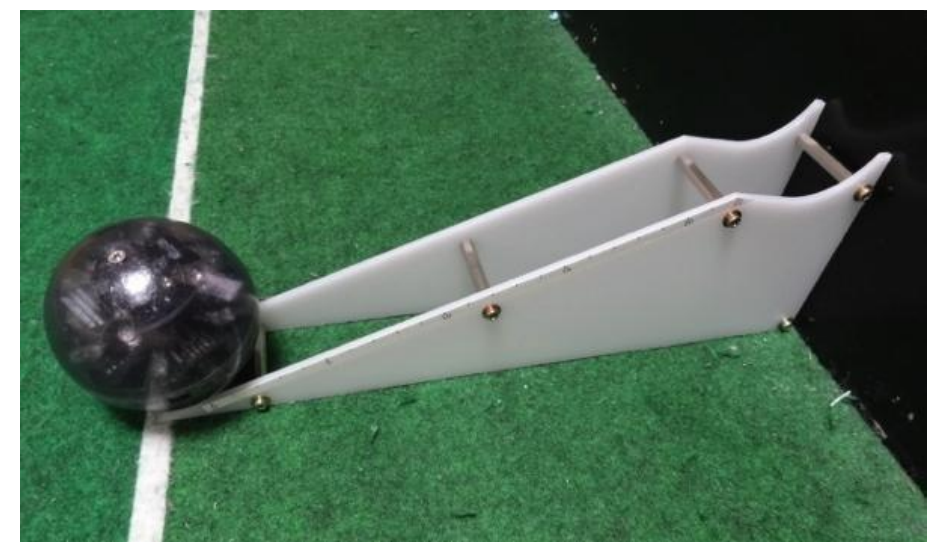
\includegraphics[width=1\textwidth]{media/image8.png}

\subsection{Materials}

\begin{table}
\begin{tabularx}{\textwidth}{
p{\dimexpr 0.64\linewidth-2\tabcolsep}
p{\dimexpr 0.36\linewidth-2\tabcolsep}}
Plastic Board & A4 paper size \\
M3 Spacers (40mm length) & 5 \\
M3 Screw & 10 \\

\end{tabularx}

\end{table}

\subsection{Device schematics}

The device schematics can be printed out from the diagram located at the end of
the document. Please be advised to check that the software you use to print the
schematic does not have a ``scale to fit'' option activated (i.e. check that it
is configured to print at 100\% or ``actual size'' scale).

Note: The device schematics shows a straight line past the 22cm mark, while the
photo shows the line at that point to be curved. Either straight or curved
lines are acceptable, but a curved line will request more difficult cutting and
the attached device schematic is simple enough for quick construction.

\subsection{Example of device construction}

\begin{enumerate}[a.]
    \item Print out the device schematics.
    \item Paste the paper on a plastic board. The incline line (red lines) should be straight.
    \item Cut out along the lines, and drill the holes.
    \item The two boards should be connected using the 40mm spacers.
\end{enumerate}

\subsection{Inspection}

\begin{enumerate}[a.]
    \item Place a ball at the bottom of the ramp run of the
        device, and put the robot in front of the ball, aiming the kicker
        towards the top of the ramp.

    \item Activate the robot's kicker for a single shot.

    \item Measure the distance that the ball traveled on the device. The
        distance should not exceed 22 cm.

\end{enumerate}

\incgraph{media/image9.png}

\section{Inspections sheet example\label{ref-065}}

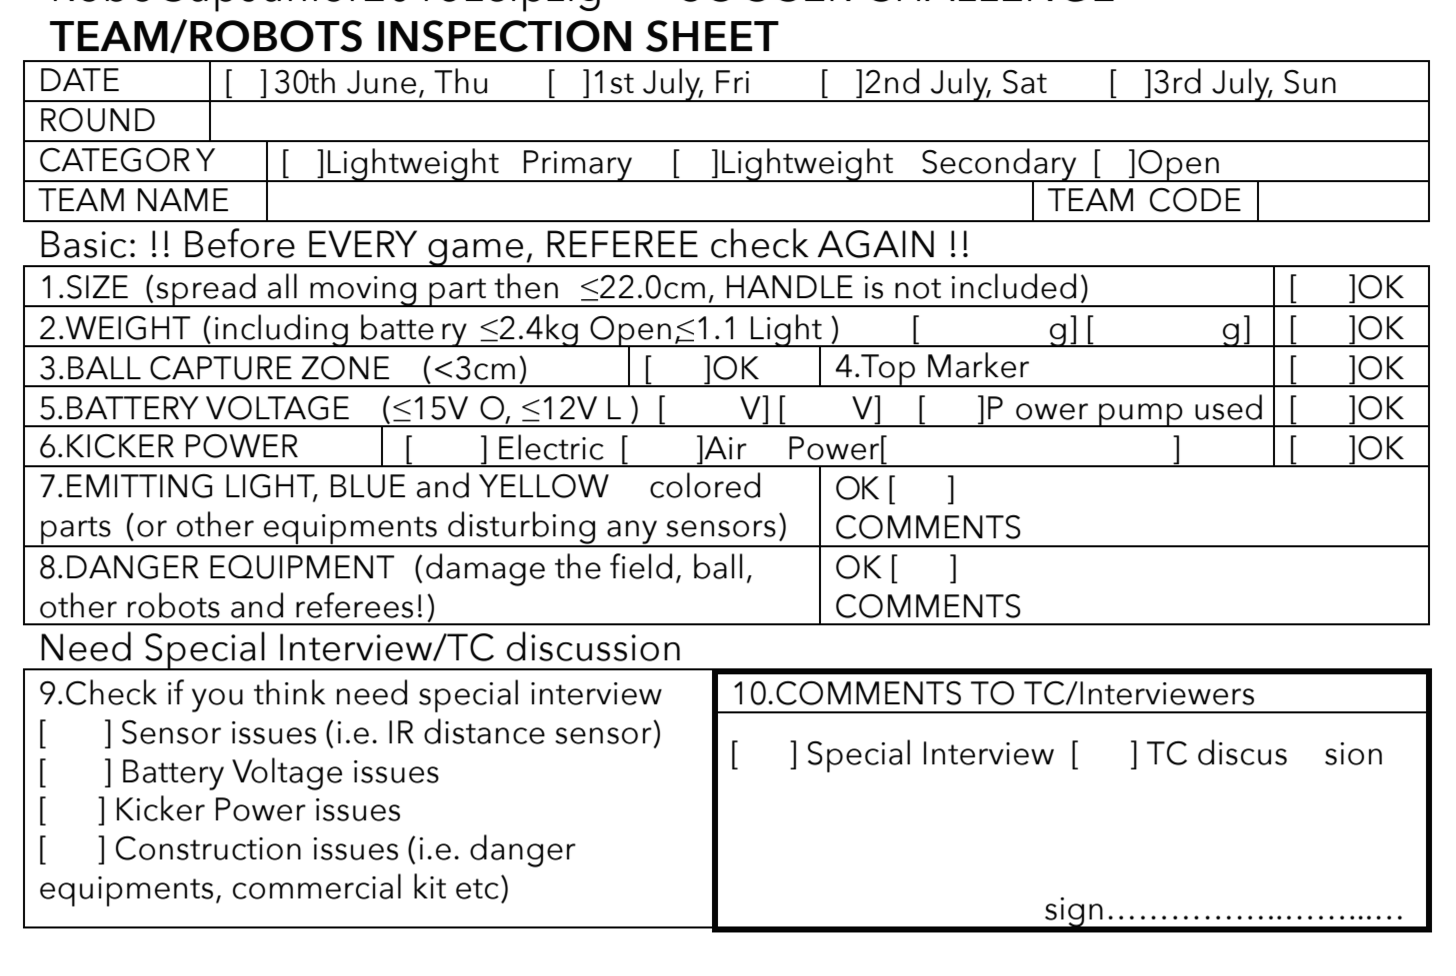
\includegraphics[width=1\textwidth]{media/image10.png}

\section{Landmarks Template (2018 version)\label{landmarks}}

The following four pages contain a template for the landmarks that are to be
put on the walls of the field. When printed on ordinary A4 paper, they should
have the measures described by these rules. While the color on the printed
papers will differ from printer to printer, printing these pages using the sRGB
``printer profile'' (color scheme) produces the best results.


\includepdf[pages=-,landscape=true]{landmarks.pdf}


\section{Landmarks Template (2017 version)\label{ref-066}}

There are colored landmarks positioned on each wall. They are 12 cm in height
and 21 cm in width. The colors used for landmarks are:

\begin{itemize}
\item Green - RGB (0, 255, 0)

\item Red - RGB (255, 0, 0)

\item Cyan - RGB (0, 255, 255)

\item Magenta - RGB (255, 0, 255)

\end{itemize}

Note that the colors were chosen so that they would be as distant from the
colors already used on the field as possible, specifically yellow and blue
which are used for goals. While both the carpet and one landmark use green as
their main color, the green used for the floor's carpet should be much darker
than the one used for the landmark.

They are positioned as follows: the green and the red one fill in the left and
the right corner behind the blue goal, while the cyan and the magenta landmarks
fill in the left and the right corner behind the yellow goal. Out of the four
walls, each of the longer ones has a combination of the landmarks used on its
edges placed in its center. See the field diagrams below for more
information.

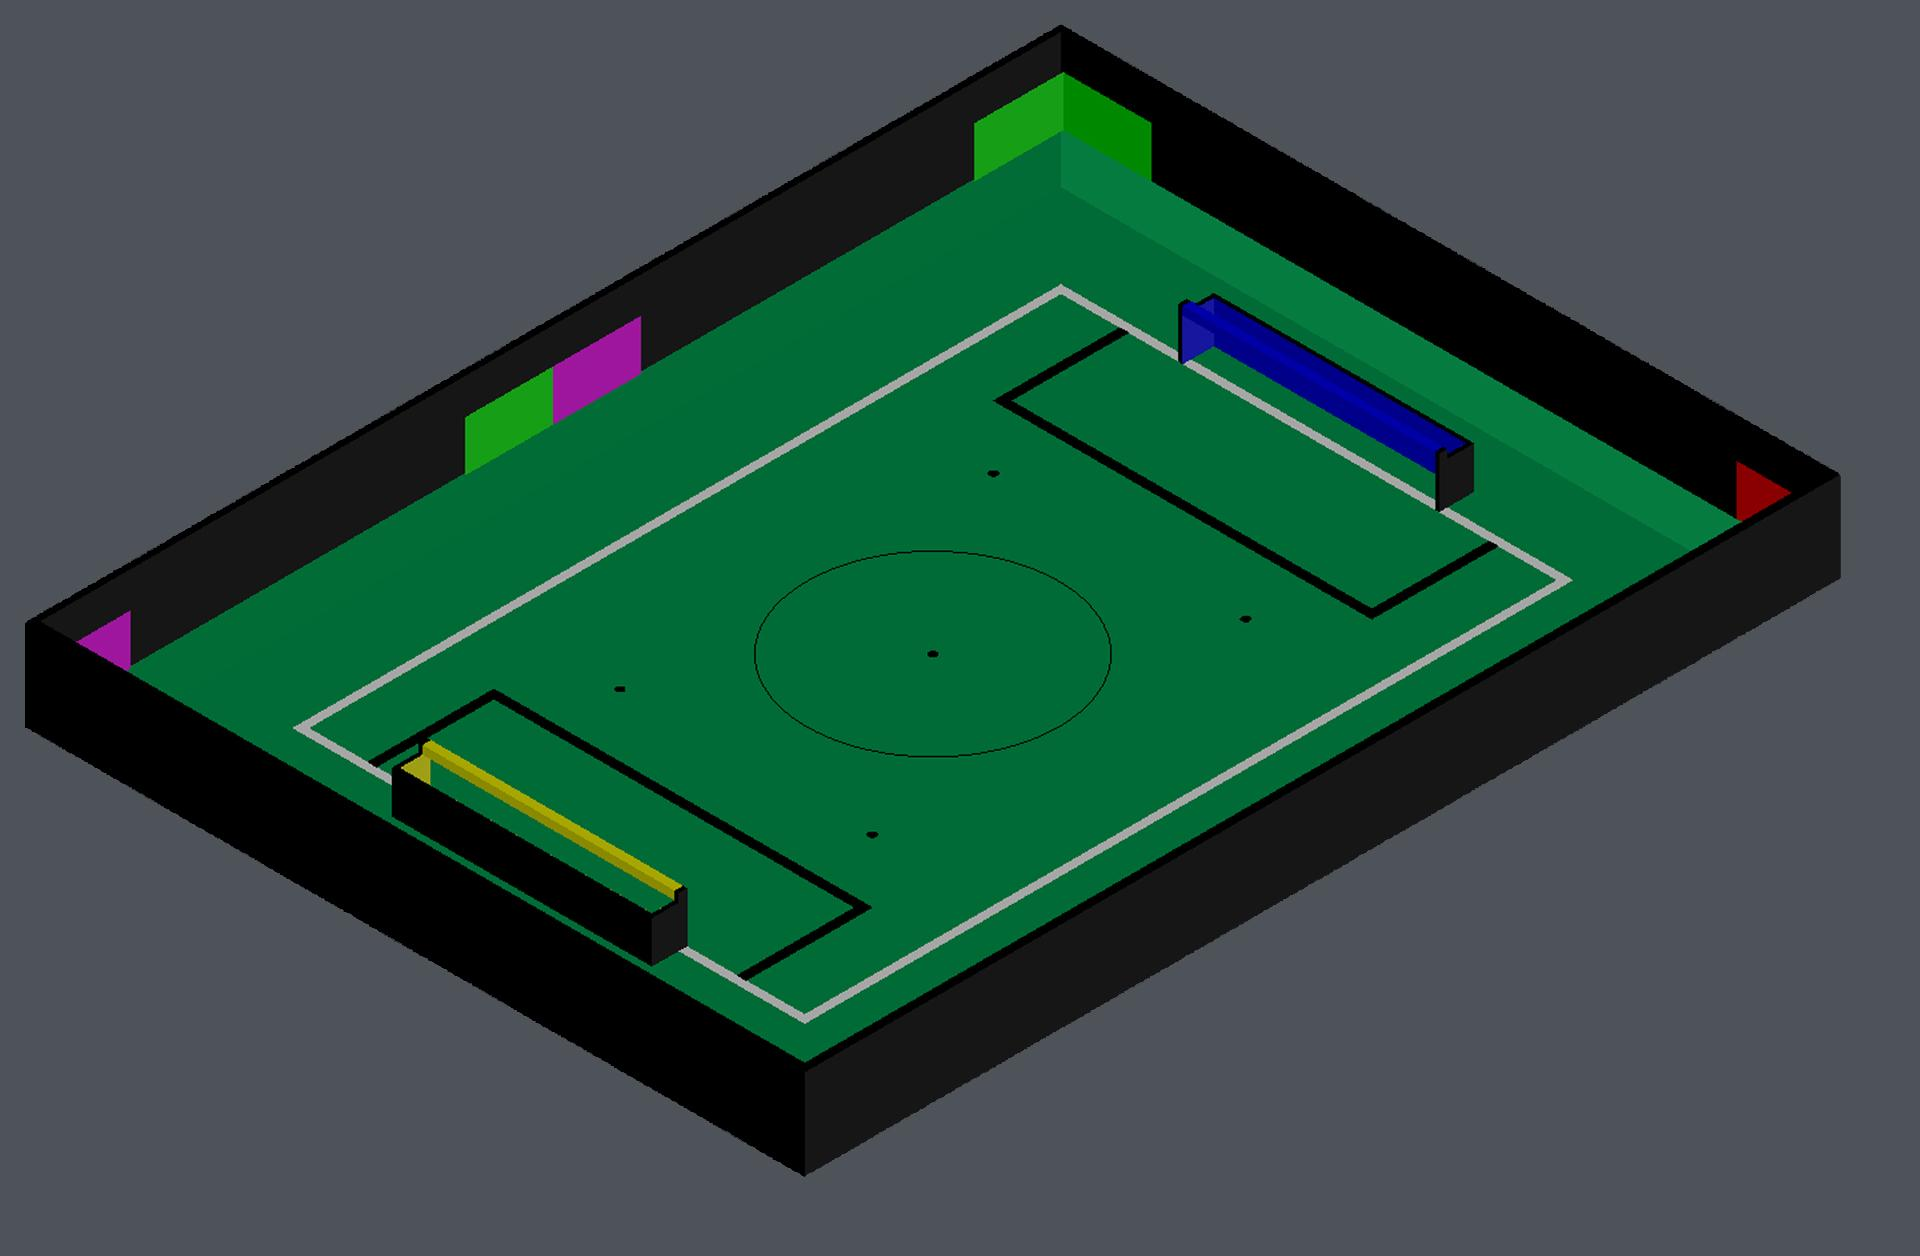
\includegraphics[width=1\textwidth]{media/image5.jpeg}
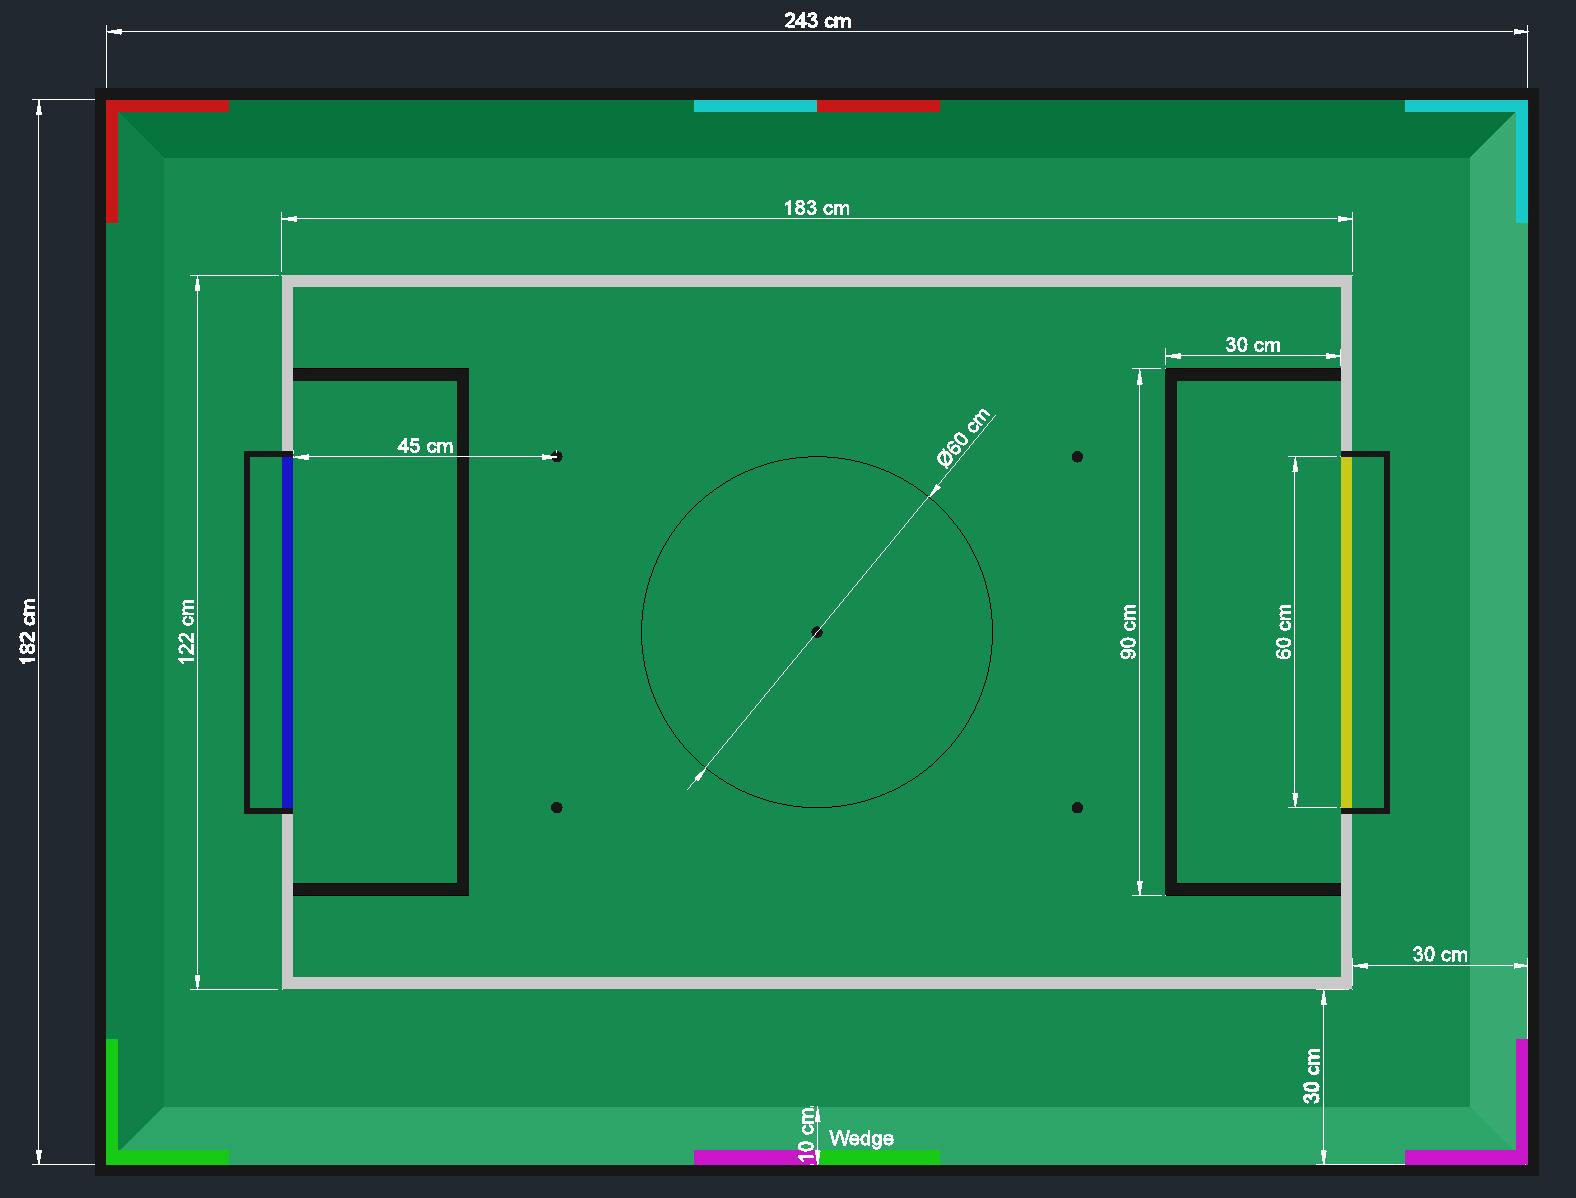
\includegraphics[width=1\textwidth]{media/image6.jpeg}
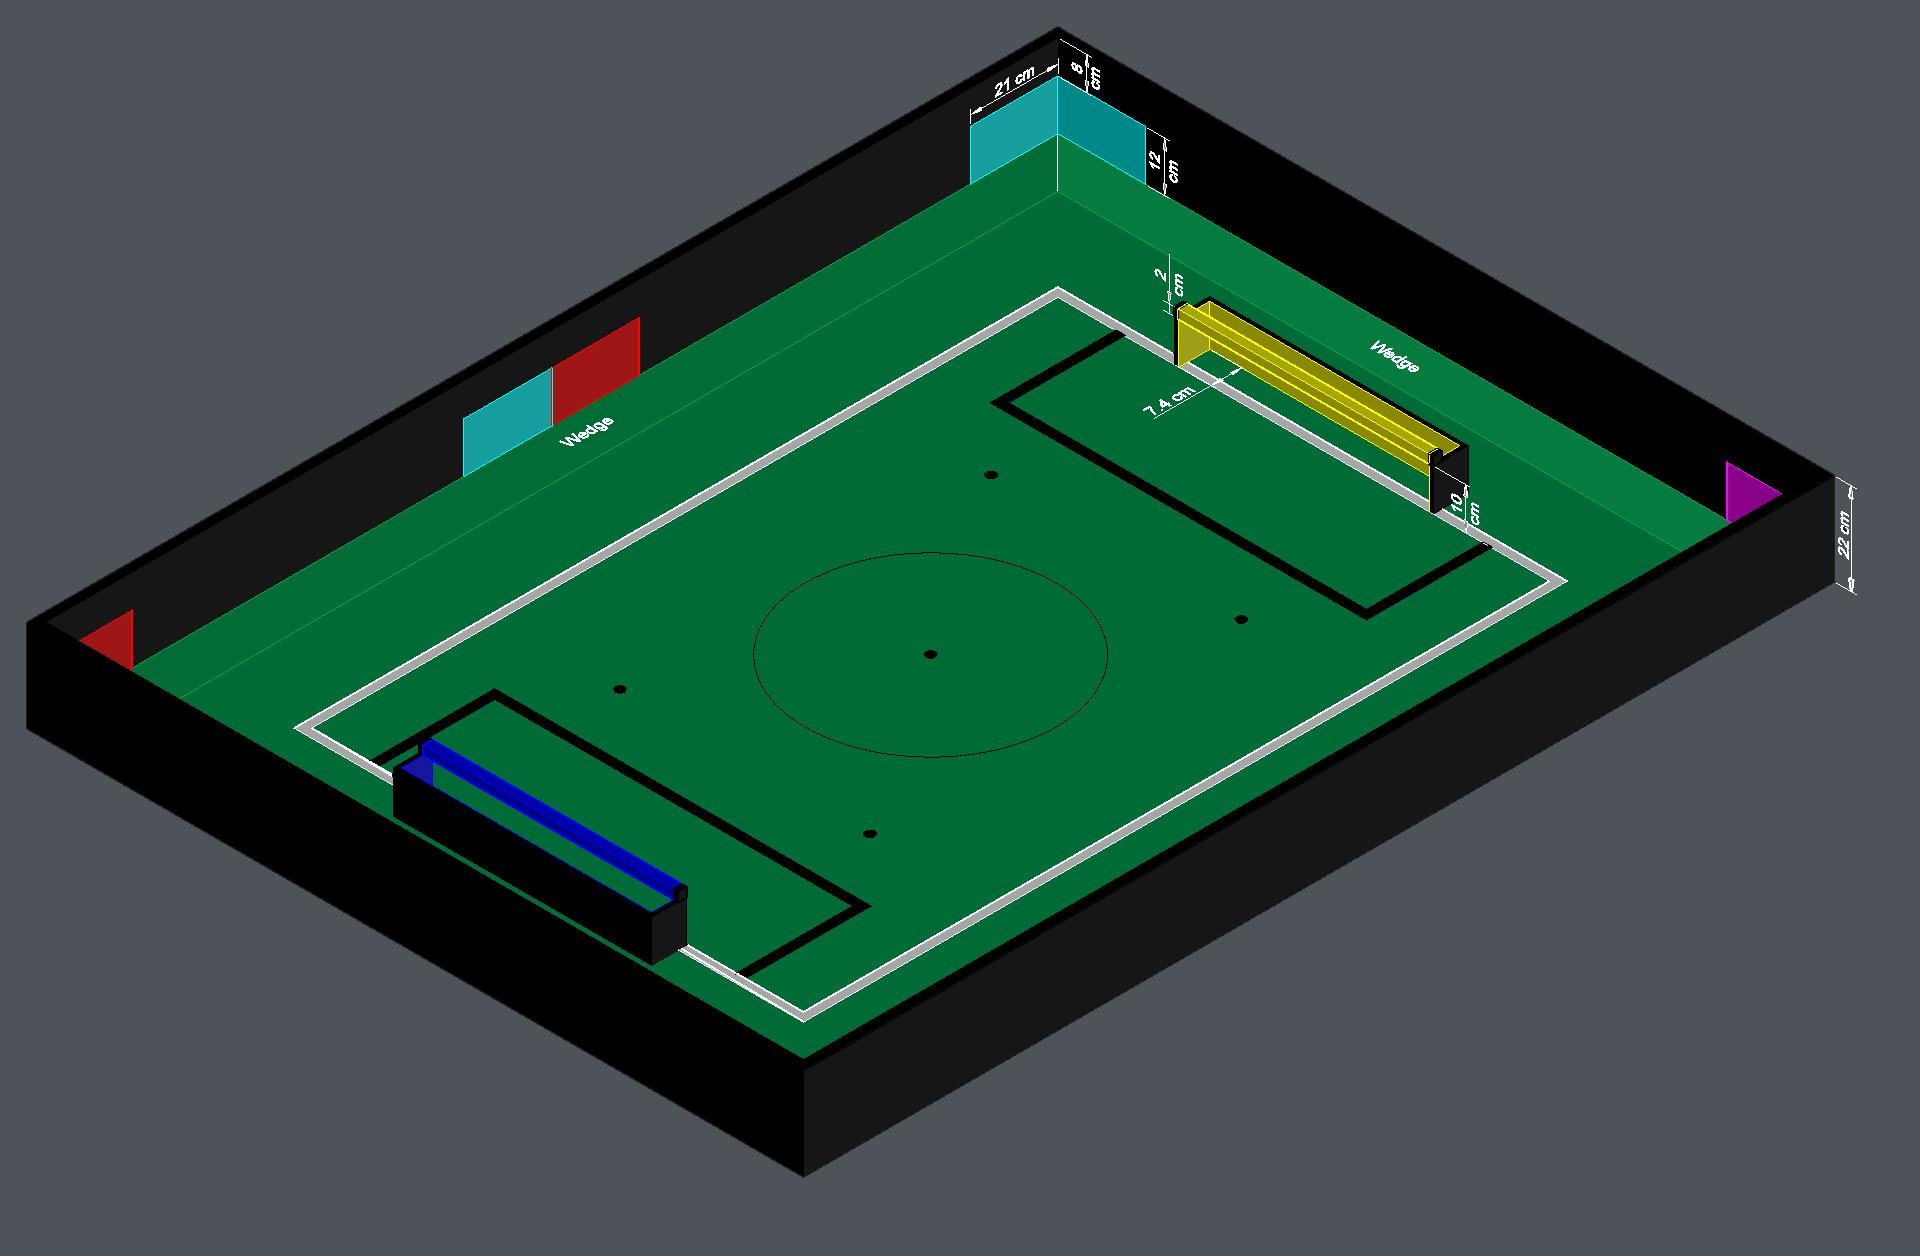
\includegraphics[width=1\textwidth]{media/image7.jpeg}

The following four pages contain a template for the \added[id=TC]{2017 version
    of} landmarks that are to be put on the walls of the field. When printed on
ordinary A4 paper, they should have the measures described by these rules.
While the color on the printed papers will differ from printer to printer,
printing these pages using the sRGB ``printer profile'' (color scheme) produces
the best results.

\newpage


\includegraphics[width=1\textwidth]{media/image11.png}


\includegraphics[width=1\textwidth]{media/image12.png}


\includegraphics[width=1\textwidth]{media/image13.png}


\includegraphics[width=1\textwidth]{media/image14.png}

\end{document}
